\subsection{Personalizacion}
Hasta ahora hemos vistos diferentes parametros para considerar los datos relevantes a nivel general, en este apartado, nos
centraremos a nivel personal.
Cada usuario es unico al igual que su situacion personal, por eso tendremos que buscar la manera de que los datos se 
adapten a los usuarios. Ofrecerle una informacion no solo relevante a nivel general pero a nivel particular.
Para ello deberemos plantearnos que necesitariamos que nos dijeran los datos en mi caso, por el lugar en el que vivo, por
mi salud, situacion familiar, algo que nos caracterize.


\subsubsection{How to solve it} 

 Estudiar en que manera los datos van a ayudar al usuario y a partir de este punto, hacerlo mas especifico, de esta manera
 pasaremos de obtener datos relevantes de manera general a ser relevantes de manera personal. Hay que pensar en el 
 usuario, no en los usuarios y buscar la manera de encontrar los resultados que se le adapten especificamente a el.

 En muchos de los casos, no podremos personalizarlo completamente, pero podemos buscar puntos comunes en subgrupos de 
 usuarios,a partir de este punto hay que estudiar las distintas casos que se pueden dar y realizar una seleccion de los que son 
 mas comunes.

 \subsubsection{How we solve it. Aire Guru} 
A todos nos interesa la polucion que nos rodea, ya que es importate para nuestra salud, por esta razon, la herramienta
Aire Guru se ha especializado en este area. Para aquellas personas que sean especialmente sensibles a la polucion del
aire, Aire Guru muestra la polucion del aire respecto a las seis condiciones medicas mas comunes que 
se ven afectadas por algun contaminante.
 

\begin{figure}[ht]
    \centering
   \subfigure[EPOC]
    {\includegraphics[width=3.5cm  ]{filter_epoc}}
    \hfill
    \subfigure [Asthma]
       { 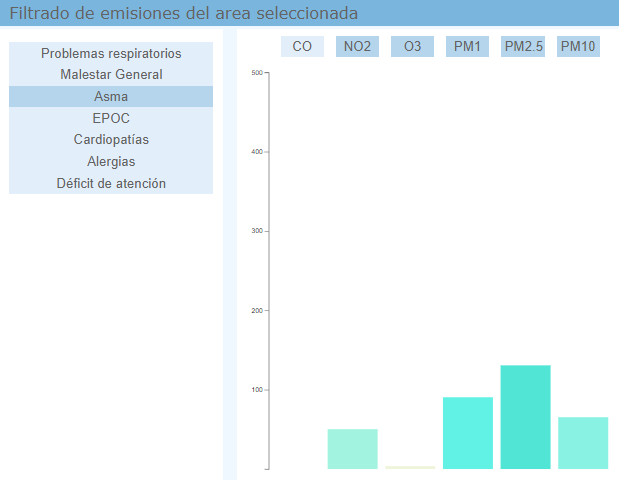
\includegraphics[width=3.5cm]{filter_asthma}}
    \hfill
     \subfigure[Allergies]
     {   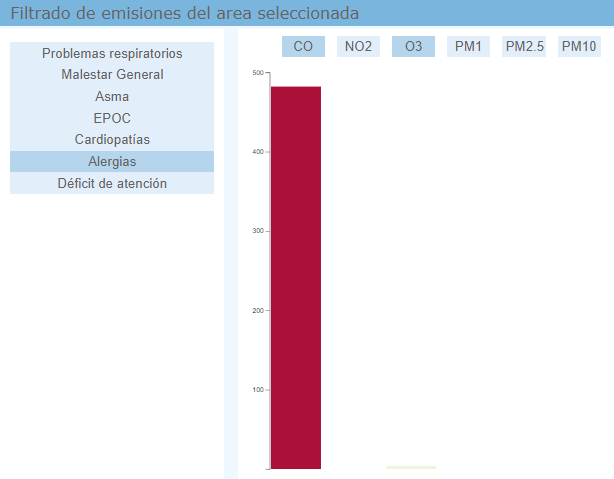
\includegraphics[width=3.5cm]{filter_allergies}}
  
  \caption{Medical Condition Filter}
    \end{figure}
 Como vemos, en cada uno de los casos, nos deberemos fijar en una seleccion de componentes.

 Otra funcionalidad de personalizacion es la representacion de la exposicion a la polucion para cada usuario. 
 Como vemos en la figura X. Personal Records, el usuario es capaz de ver la polucion que le ha rodeado especificamente
 a el a lo largo del tiempo.

 
\elsparagraph{Evaluation}  
\begin{itemize}
    \done El usuario cuenta con funcionalidades especializadas 
    \crossed La funcion del filtrado de la condicion medica no se autoselecciona, esto es debido a que la funcionalidad
    esta disponible para todos los usuarios. Podria implementarse de manera que el mapa mostrara el AQI con respecto a los
    contaminantes que el usuario ha preseleccionado, pero esto puede llegar a desvirtualizar la informacion si no se 
    indica al usuario claramente, que el mapa no toma en cuenta todos los contaminantes relevantes.
\end{itemize}
 \newpage